
\documentclass[a4paper,12pt]{article}
\title{projectreport}
\usepackage[top=1in, bottom=1in, left=1in, right=1in]{geometry}
\usepackage{epsfig}
\usepackage[nottoc]{tocbibind}
\usepackage{float}
\usepackage{multicol}
\usepackage{graphicx}
\usepackage{titlesec}
\usepackage{lipsum}
\usepackage{caption}
\usepackage{subcaption}
\usepackage{booktabs}
%\usepackage[dvips]{graphics}
\usepackage{sectsty}
\usepackage{chngcntr}
\usepackage[hidelinks]{hyperref}
\usepackage{algorithmic}
\usepackage{algorithm2e}

%\usepackage[dvips]{graphics}
\sectionfont{\centering}
%\usepackage{helvet}
%\renewcommand{\familydefault}{\sfdefault}
%\usepackage{titlesec}
%\setkomafont{section}{\normalfont\huge\sffamily\bfseries\color{blue}}
%\renewcommand{\rmdefault}{phv} % Arial
%\renewcommand{\sfdefault}{phv} % Arial
\renewcommand{\abstractname}{\large Abstract}
\counterwithin{figure}{section}
\newcommand*{\myfont}{\fontfamily{Arial}\selectfont}
\renewcommand{\baselinestretch}{1.5}


\begin{document}

\pagenumbering{gobble}
\thispagestyle{empty}
\begin{center}
\textit{Major Project Report on} \\
\vspace{2 mm}
\Large{\textsc{ Remote OS Image cloning and  deployment management }}   % Your major Project Title

\vspace{7 mm}
\large{\textbf{                  % Group members name
Gaurav U D ( 16IT113 )  
\\Abhilash V ( 16IT201 )   
\\Rahul A R ( 16IT239 ) 
}}
\\
\vspace{4 mm}
Under the Guidance of,\\
\textbf{Dr Jaidhar C D}\\         % Name of your guide
Department of Information Technology, NITK Surathkal\\
\vspace{4 mm}
\textit{Date of Submission: 01/10/2019}
\\
\vspace{4 mm}
in partial fulfillment for the award of the degree
\\
%\vspace{3 mm}

of

\textbf{Bachelor of Technology}

In

\textbf{Information Technology}

At
\vspace{4 mm}
	
		
\includegraphics[width=1.5in,height=1.5in]
		{nitk.jpg}
 
\textbf{Department of Information Technology}

\textbf{National Institute of Technology Karnataka, Surathkal}

\textbf{October 2019}
\end{center}

%%%%%%%%%%%%%%%%%%%%%%%%%%%% Page 2 %%%%%%%%%%%%%%%%%%%%%%%%%%%%%%%%%%%%%%
\newpage

\begin{center}
\textbf{\large{Department of Information Technology, NITK Surathkal}} \\

\textbf{\large{Major Project}} \\
\textbf{\large{Mid Semester Evaluation Report (October 2019)}} \\
\noindent\rule{12cm}{0.4pt}
\end{center}


\noindent
\textbf{Course Code :} IT 449 \\
\textbf{Course Title:} Major Project \\
\textbf{Project Title:} \emph{Remote OS Image cloning and  deployment management}   % update project title

\subsubsection*{Project Group:}
\begin{tabular}{lcl}
\hline                         % Update name of students here 
Name of the Student & Register No. & Signature with Date 			\\
\hline
Gaurav U D			&16IT113		&							\\\\
Abhilash V			&16IT201		&							\\\\
Rahul A R			&16IT239		&							\\\\
\hline
\end{tabular} 

\vspace{5 em}

Place:

Date:\hfill \textit{(Name and Signature of Major Project Guide)}


%%%%%%%%%%%%%%%%%%%%%%%%%%% Page 3 %%%%%%%%%%%%%%%%%%%%%%%%%%%%%%%%%%%%%%


\newpage
         \begin{abstract}
Every computer lab session has its own set of requirements and software to be installed. Manual installation and maintenance of this software is a tedious task. Hence this project aims to develop a computer imaging solution which can capture OS images with all the required software pre-installed and deploys these images on the individual client systems.
The bare-metal client systems boot after connecting to the network using PXE (Preboot Execution Environment). The client can then choose an OS image they want to deploy,  from the available OS images from the server. Alternatively, the administrator can also deploy the images on each individual client machine. The OS image is then sent to the client machine which installs it in its local hard disk and then reboots using the newly installed OS.



% \textbf{Keywords:  }\emph{your keywords }
	\end{abstract}

%%%%%%%%%%%%%%%%%%%%%%%%%%% Page 4 %%%%%%%%%%%%%%%%%%%%%%%%%%%%%%%%%%%%%%

\newpage
\tableofcontents

%%%%%%%%%%%%%%%%%%%%%%%%%%% Page 5 %%%%%%%%%%%%%%%%%%%%%%%%%%%%%%%%%%%%%%

\newpage
\listoffigures

%%%%%%%%%%%%%%%%%%%%%%%%%%% Page 6 %%%%%%%%%%%%%%%%%%%%%%%%%%%%%%%%%%%%%%

\newpage	
        
\pagenumbering{arabic}

%%%%%%%%%%%%%%%%%%%%%%%%%%% Page 7 %%%%%%%%%%%%%%%%%%%%%%%%%%%%%%%%%%%%%%

\section{\fontsize{16pt}{1em} \usefont{T1}{phv}{b}{}Introduction}
Each computer lab session has its own set of requirements in terms of the needed software and type of Operating System (OS). The traditional method is to install the required OS through USB to individual computers. If each lab session has different OS and software requirements, then this method is inefficient as it requires more time and manual intervention.
\paragraph{}
Remote OS image deployment refers to deploying the image stored on a remote server on to bare metal client computers with no or little software initially on the hard disk,  connected to a LAN  network. The image here refers to a “disk image” which contains OS along with its root file system and other partitions of the disk. 
In each lab session, computers ( clients attached to LAN ) boot to the menu containing a list of available OS images and the client chooses one among them to be deployed. The image is then deployed from the remote server on to the client machine, and the client reboots to the deployed OS. Lab administrator may first install an OS with required software on a computer and make an image of the system, which can then be placed in a storage server and through this deployment process, it can be installed on all clients. If any of the students corrupt the computers (clients), he/she need to reboot the system and deploy the image again from the server for precise installation. 
\vspace{0.5cm}

\newpage
\section{\fontsize{16pt}{1em} \usefont{T1}{phv}{b}{} Literature Survey}


\subsection{\usefont{T1}{phv}{b}{it} Related Work}

Web-Based Computer Lab Imaging with Grimiore [1] provides a web-based frontend for the disk imaging software Clonezilla. Grimoire allows administrators to restore and maintain an entire lab of computers, rather than a single computer or a single homogeneous image. Administrators can create a lab configuration for each use of the lab and restore them with a single option. Grimiore stores configuration data for each computer in each class, allowing lab configuration to contain heterogeneous images. Finally, Grimiore is web-based and provides administrative control over the entire imaging system, as well as user-level control over a single client computer.
This project handles the management side of Clonezilla and does not focus on the implementation.
\paragraph{}
Network enters Highly-Efficient Management Solutions based on Intel PXE-
based Remote Cloning System [2] uses PXE boot and multicast technology for cloning and imaging. The paper explains in detail about PXE technology, the basic protocols it supports and setting up of PXE enabled servers in the Windows2000.
It uses Norton Ghost cloning software, which is now proprietary software. The tool supports multicast, i.e. sends the image once from the server for deployment to all the clients in the multicast session. Their system adopts NTFS file system at the storage node as it provides a large capacity of file storage, making the storing of image files ( greater or equal to 4GB) more convenient. This work uses many proprietary software components to build the system, and the work is mostly based on how to set up and integrate Norton Ghost Multicast technology for cloning and imaging system with little or no focus on improving the existing system on multicasting of images through the network. It also does not mention the design of the image management system in a software view, i.e. various functionalities that provide for administrator and students.
\paragraph{}
Fog project [3] is an open-source cloning and image management solution. Administrator initiates image deployment on a single computer or multiple computers by means of a web interface[4]. The client can choose and initiate image deployment using PXE(Preboot Execution Environment)[5]. Regardless of  the way of initiating the deployment, client is booted from the PXE network, the deployed image is downloaded from the remote server and deployed to client local hard disk through any one of the cloning utilities like partclone[6] or partimage[7] which are included in the tiny operating system. IPXE[8] software is used as the bootloader which boots to tiny Linux based operating system (minimal kernel and file system, which has image cloning utilities) downloaded from the network and deploys the image from storage node (remote server containing the images). It also supports both unicast and multicast ways of image deployment. Fog project achieves multicasting through Linux based tool called Udpcast. It does not support client-oriented image capture and saving of client files between imaging.
\paragraph{}
Partimage is open-source disk backup software. It saves partitions having a supported file system on a sector basis to an image file. The image file is compressed to save disk space and transfer time and is split into multiple files. Partimage only copies data from the used portions of the partition, i.e. free blocks are not written to the image file. This is unlike other commands like 'dd', which also copy unused blocks. This increases the speed of image restoration and results in more space-efficient backup. It does not support 'ext4' or 'btrfs' filesystems.
Partclone is an open-source software similar to  Partimage. Partclone provides utilities to save and restore used blocks on a partition and is designed for higher compatibility of the file system by using existing libraries. It also supports 'btrfs' and 'ext4' filesystem in addition to what Partimage supports.
For example, if partition size is 10 GB but only 5 GB is used, Partclone or Partimage clones only 5GB and compresses it. It can then deploy the image to hard disk having space of atleast 5GB.
\subsection{\usefont{T1}{phv}{b}{it} Outcome of Literature Survey}
In labs, the requirement is to have different OS/software or both for each lab session. Hence there is a need for frequent imaging, and sometimes the same set of OS/software is needed multiple times. For example, subject A requires specific software and OS, and during each session of subject A lab, that particular OS image needs to be installed and used, i.e. the same image is being used by the subject A lab periodically. Fog project always downloads the image through the network and deploy it. It does not exploit the fact that the same image is being reused periodically to optimise image transfer from the network, i.e. does not have a cache-like mechanism to prevent re-downloading of the same image.
\paragraph{} 
None of them allows the client to capture its own image for further use, as it would increase the storage size on the storage node. Also,  the projects do not provide any mechanism for client files to be saved between imaging, i.e. the work done by the client in the lab persists until the next imaging takes place. Fog provides only provides some scalability mechanism to handle the deployment of images to a large number of clients.  
\paragraph{}
Partclone supports cloning for more file systems than the partimage. Both of them support cloning and imaging of only used portions of partition, unlike 'dd' command. They can create a clone and deploy a larger partition image to a smaller partition space but with inconsistency. It needs to be used along with a partitioning tool to resize the partition.
\paragraph{}
 Making the system as open-source leads to easier adoption  in educational institutions, gives platform for more development and making the system more features rich and end consumer-oriented. 

\subsection{\usefont{T1}{phv}{b}{it}Problem Statement}
Aim is to design and develop an efficient OS image cloning and deployment system where bare metal client systems can boot from remote OS images

\subsection{\usefont{T1}{phv}{b}{it}Objectives}
\begin{enumerate}
\item  To deploy OS images remotely on bare metal clients.
\item To support Client driven deployment i.e. client has the ability to choose the required image to be deployed
\item To develop a user interface for the administrator to manage image capture and deployment
\item To optimize the process of image capture in terms of space and time
\item To develop a mechanism for time optimised large scale unicast and multicast frequent deployment of images 
\end{enumerate}


\newpage
\section{\fontsize{16pt}{1em} \usefont{T1}{phv}{b}{}Requirements}
We have identified the necessary requirements for Remote OS cloning and image deployment system to be functional as a product that can be used for labs. We have classified the requirements as user and system requirements, user requirements are summarised in the use case diagram in fig 3.1
\subsection{\usefont{T1}{phv}{b}{it}User requirements}
\begin{enumerate}
\item Automate without any manual intervention in installing OS having specific software.
\item In the lab, the requirement is to have different OS  /software or both for each lab session, i.e. there is a need for frequent imaging and also the same set of OS/software needed after some period.
\item Easy to set up and manage image capture and deployment ( admin point of view) system.
\item Keeping one of the storage partitions unaffected by imaging in a client machine, where the clients can store the files.
\item Both client and the lab admin can capture and store images. The client may have installed and configured new software, he/she may want to use the same configured OS, the next time he/she comes to that lab, i.e. they have to have the ability to capture the OS image and then restore it whenever needed.
\item Give support for both Windows and Linux based distribution OS images.
\item Give support to heterogeneous environment of UEFI and BIOS firmware based clients.
\end{enumerate}
\subsection{\usefont{T1}{phv}{b}{it}System requirements}
\begin{enumerate}
\item client needs to be PXE enabled, and no other client setup is required
\item Network connectivity through LAN cable.
\item Availability of servers to set up DHCP, TFTP and storage servers
\item Integrate the DHCP server required by this system to an existing DHCP server.
\end{enumerate}
\begin{figure}[h!]
    \centering
    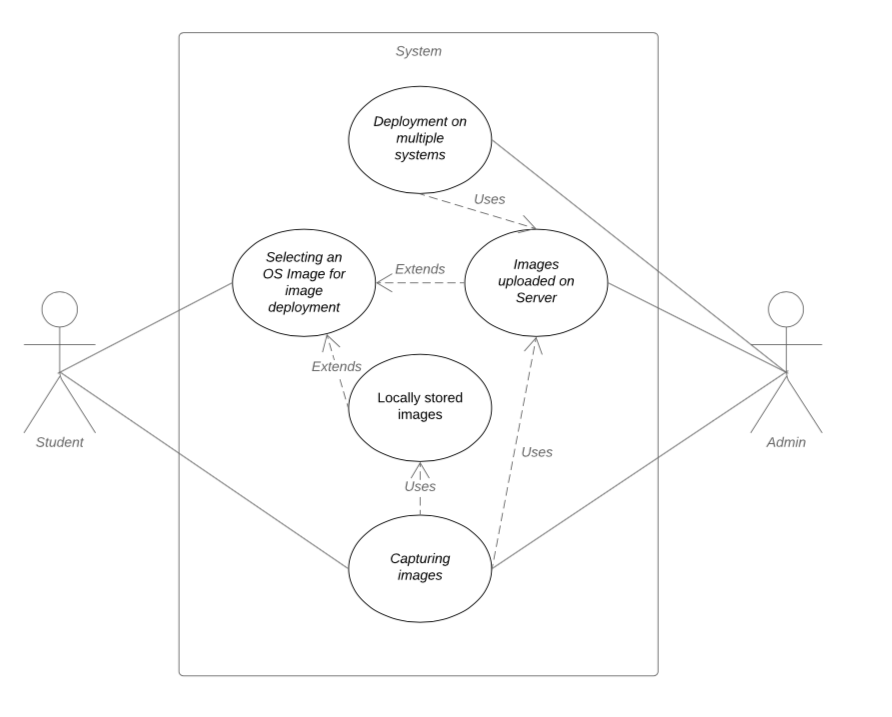
\includegraphics[width=\linewidth]{i1.png}
    \caption{Use Case diagram of the system}
    \label{fig:Use case}
    \small
    ( Student chooses the image to be deployed from the central server or local harddisk
    Administrator maintains the central repository of images and can deploy
    images to any of the clients remotely )
\end{figure}

% \begin{enumerate}
%     \item Student has to choose the image which he/she wants to deploy,
%         \begin{enumerate}
%             \item Has to choose the image which he/she wants to deploy from either the local harddisk or the central server
%             \item Can make certain changes to the OS and save it locally after capturing for further use
%         \end{enumerate}
%     \item Administrator
%         \begin{enumerate}
%             \item Maintains the central repository which has all the images
%             \item Can deploy images to any of the clients remotely
%         \end{enumerate}
% \end{enumerate}


\newpage
\section{\fontsize{16pt}{1em} \usefont{T1}{phv}{b}{}Methodology}
Remote OS cloning and image deployment system orchestrates the image deployment through the collection of server interaction without any initial client software except for PXE enabled client, i.e. bare-metal client. It is difficult to clone the disk from inside the existing  OS of the client as it requires for the file system to be unmounted and also image deployment from within existing OS in the client will lead to inconsistencies. So the bare-metal client is used for imaging. The required software such as bootloader and the image deployment tool is loaded from network to memory through PXE booting.
\subsection{\usefont{T1}{phv}{b}{it} PXE Boot}
PXE ( Preboot Execution Environment) technology allows a client to boot from network loaded operating system through support of PXE enabled servers. PXE technology is a firmware that supports industry-standard Internet protocols, namely UDP/IP, DHCP and TFTP. It is present in all Intel-based computers, but it needs to be PXE enabled and connected through LAN cable to a network containing PXE enabled servers. 
PXE enabled servers refers to a set of servers which supports PXE client specifically for PXE boot. It contains the following components summarised in fig 4.1 : 
\begin{enumerate}
 \item DHCP server: It assigns the IP address to LAN PXE client, gives the name of boot file and location (IP address) of TFTP server to access it in addition to normal DHCP servers which only assigns the IP address.
 \item  TFTP server: It stores boot files (bootloader and OS)  which  PXE client downloads after IP assignment. TFTP is used be because it is easily implemented in the client's NIC firmware, resulting in standardized small-footprint PXE ROMs
 \item  Network Bootloader and OS : A Network bootloader to be able to boot a tiny network OS from the network ( Contains the image cloning and deployment tools). Both of them are present on the TFTP server.
 \end{enumerate}
 The PXE client network boots by connecting to a network and requests an IP address and the location of the bootloader. The DHCP server assigns an IP address and sends boot file name along with the IP address of TFTP server. The PXE client then retrieves the grub modules from the TFTP server and loads grub, the grub boots into a tiny operating system located on the TFTP server.
 \begin{figure}[h!]
    \centering
    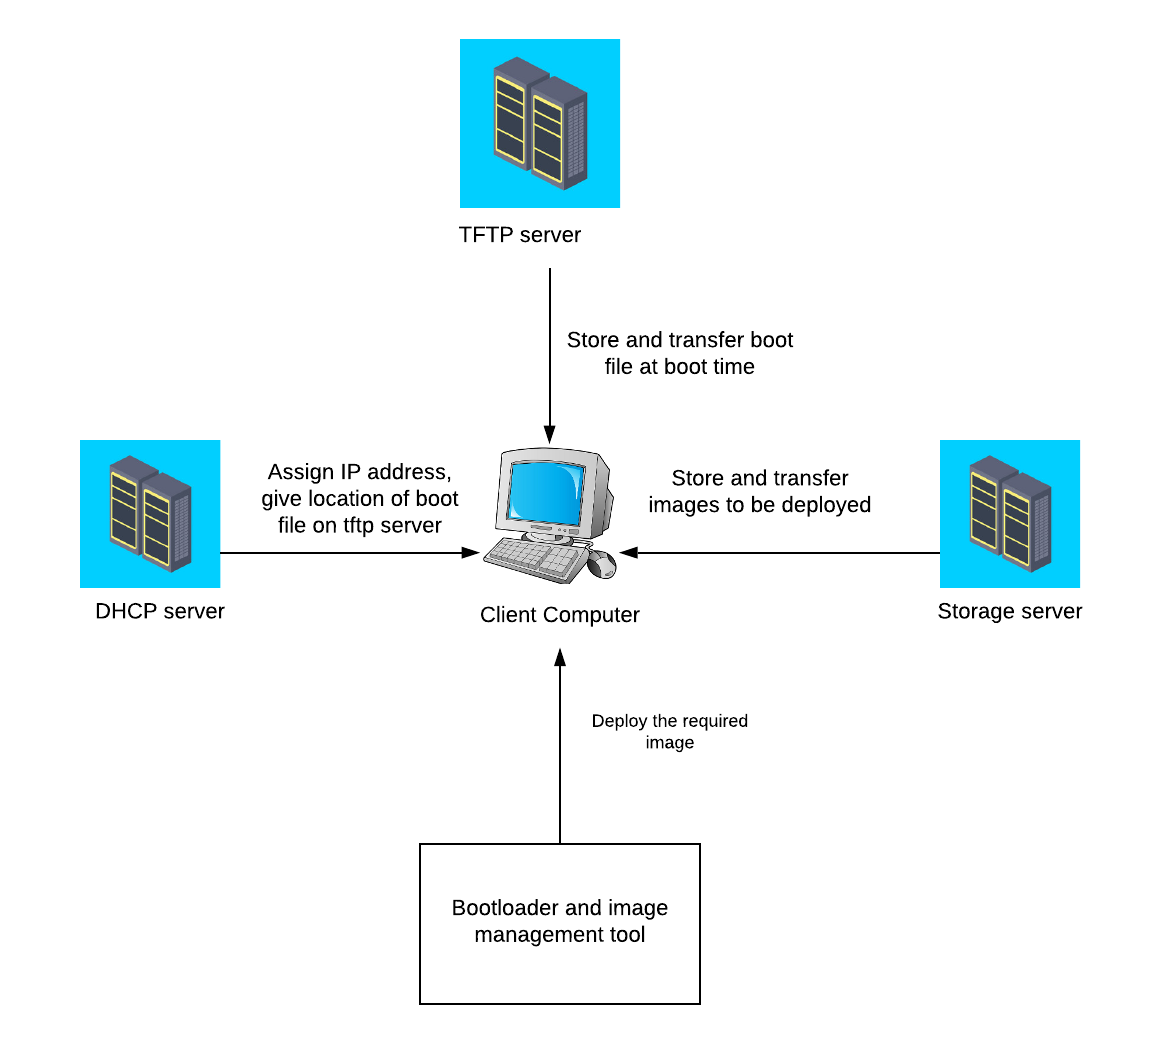
\includegraphics[width=\linewidth]{architecture.png}
    \caption{Basic System Architecture}
    \label{fig:Use case}
\end{figure}
\newpage

% 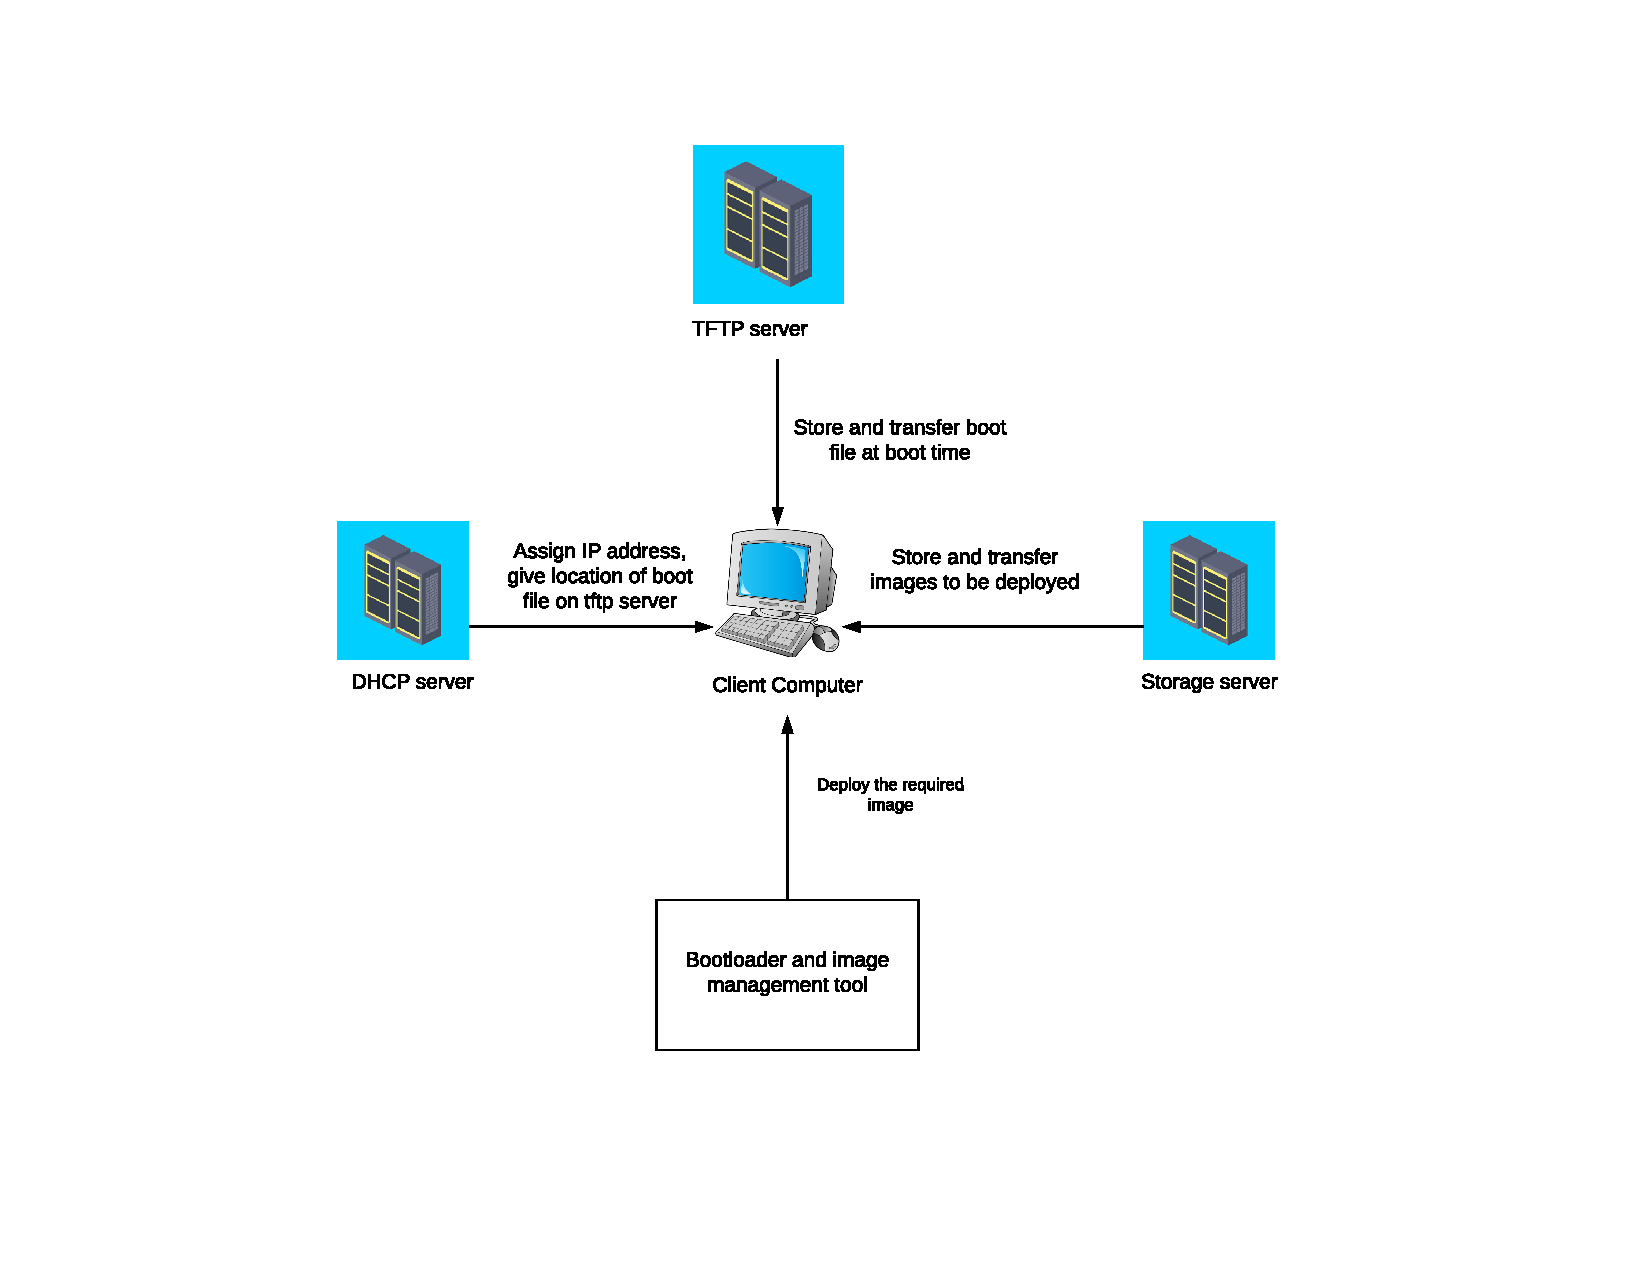
\includegraphics[page=1, trim = 18mm 80mm 18mm, clip, width=14.35cm]{basicsysarch.pdf}
% \captionof{figure}{Basic System Architecture} 
\subsection{\usefont{T1}{phv}{b}{it} Remote Image cloning and Deployment System}
  The network booted OS contains tools for cloning and imaging. A storage server is needed to store cloned images. It is used in the fast transfer of images from the server to the client during deployment and from client to server during cloning.
  The tiny operating system displays a menu ( if its not deployed by the admin ) of available images on the storage server, and when a choice is made by the client, that particular image is downloaded from the storage server and then deployed. Then the system reboots directly to the deployed image. A web interface is designed to handle all the operations at the admin side.
  Entire workflow is summarised in flowchart fig 4.2
%\\
%  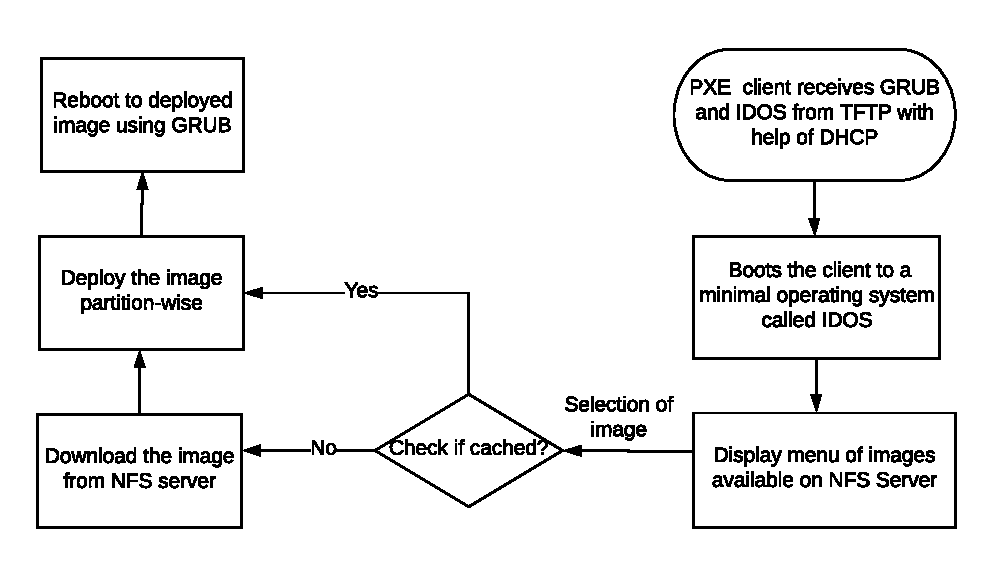
\includegraphics[page=1, trim = 18mm 80mm 18mm, clip, width=14.35cm]{Workflow.pdf}
%  \\
%  \\
%  \\
\newline
\begin{figure}[h!]
    \centering
    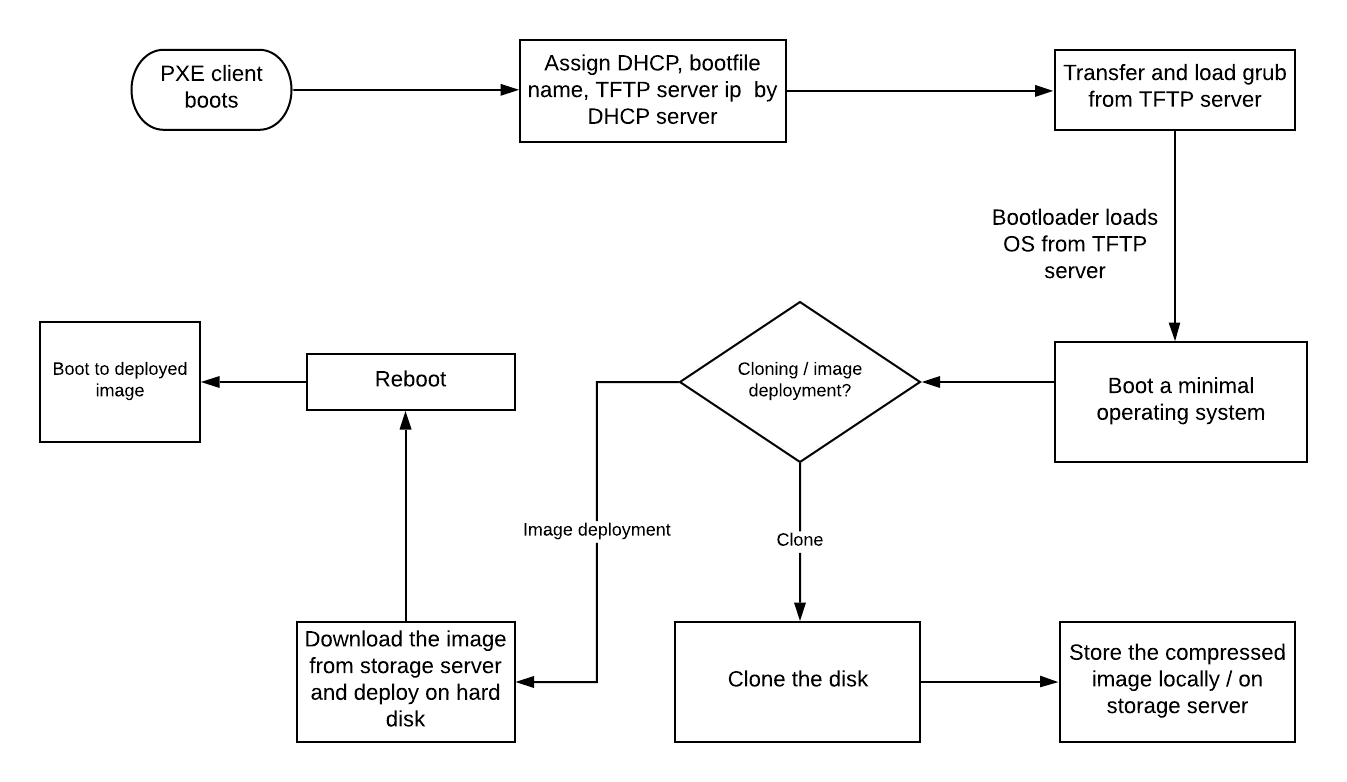
\includegraphics[width=\linewidth]{Workflow.png}
    \caption{Flowchart of remote OS image cloning and deployment system}
    \label{fig:Use case}
\end{figure}
% \captionof{figure}{Flowchart of remote OS image cloning and deployment system } 
%  \newpage
% \section{\fontsize{16pt}{1em} \usefont{T1}{phv}{b}{}Work Done}



% \newpage
% \section{\fontsize{16pt}{1em} \usefont{T1}{phv}{b}{}Results and Analysis}


% \newpage
% \section{\fontsize{16pt}{1em} \usefont{T1}{phv}{b}{}Conclusion \& Future Work}
\newpage
\section{\fontsize{16pt}{1em} \usefont{T1}{phv}{b}{}Timeline}
 \begin{figure}[h!]
    \centering
    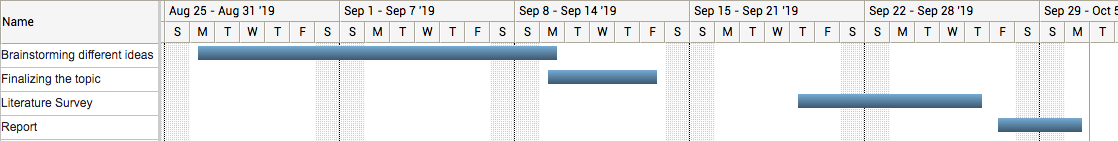
\includegraphics[width=\linewidth]{ganntt.png}
    \caption{Timeline of work done till now}
    \label{fig:Use case}
\end{figure}


%create bibtex files for references
\newpage
\bibliographystyle{plain}
\bibliography{references.bib}
\begin{enumerate}
    \item Josh A. Meek, Michael K. Bradshaw et al. Web Based Computer Lab Imaging with Grimiore. In Proceedings of the 37th annual ACM SIGUCCS fall conference: communication and collaboration ( 2009 ) doi: 10.1145/1629501.1629507
    \item Li linhui, Zhang Ke, Zhang Fang et al. Network Center's Highly-Efficient Management Solutions based on Intel PXE-based Remote Cloning System.
    In 3rd International Conference on Advanced Computer Control (ICACC 2011)
    \newline
    doi: 10.1109/ICACC.2011.6016442
    \item \href{https://fogproject.org/}{FOG Project} - A free open-source network computer cloning and management solution
    \newline
    \url{https://fogproject.org/}
    
    \item Wikipage of FOG project
    \newline
    \url{https://wiki.fogproject.org/}
    \item PXE - Preboot execution environment
    \newline
    \url{https://en.wikipedia.org/wiki/Preboot_Execution_Environment}
    \item Partclone - Partition clone and restore tool
    \newline
    \url{https://www.partclone.org/}
    \item Partimage - Open source disk backup software
    \newline
    \url{https://www.partimage.org/}
    \item IPXE - Open source network boot firmware
    \newline
    \url{https://ipxe.org/}

\end{enumerate}

\end{document}